\chapter{Resultados \label{chap:Resultados}}
%%%%%%%%%%%%%%%%%%%%%%%%%%%%%%%%%%%%%%%%%%%%%%%%%%%%%%%%%%%%%%%%%%
%%%%%%%%%%%%%%%%%%%%%%%%%%%%%%%%%%%%%%%%%%%%%%%%%%%%%%%%%%%%%%%%%%
\section{Ajuste de espectros}
\noindent Habiendo calculado y aplicado los valores de expectación, $\mu_{g}$ y $\mu_{bkg}$, para corregir la carga sobre los clusters y habiendo introducido el modelo de la colección parcial de carga, usado en los ajustes de los espectros, ya se pueden obtener los resultados derivados de las correcciones.

Los resultados que se presentan a continuación son tanto para el pico del flúor como los picos del aluminio. Para ambos casos se muestran los histogramas con sus respectivos ajustes para cada uno de los pasos del análisis con el fin de poder comparar los resultados de unos con otros: Primero utilizando el umbral \verb|EPIX = 0.5|, luego aumentando el umbral a \verb|EPIX = 1.5| sin aplicar las correcciones y, por último, los resultados con el umbral \verb|EPIX = 1.5| aplicando las correcciones. Todos los resultados que se presentan son para el primer cuadrante del sensor.

\subsection{Fluor}
\noindent Para el caso del pico del flúor, se tiene en el gráfico de la Figura \ref{fig:F_OHDU0_EPIX05} el ajuste del histograma de carga con \verb|EPIX=0.5|. Se puede observar como el modelo ajusta muy bien los datos. Además es importante destacar la cantidad de eventos que contabilizó el algoritmo de clusterización (\verb|skExtract|) fue $2379$. 
\begin{figure}[h]
    \centering
        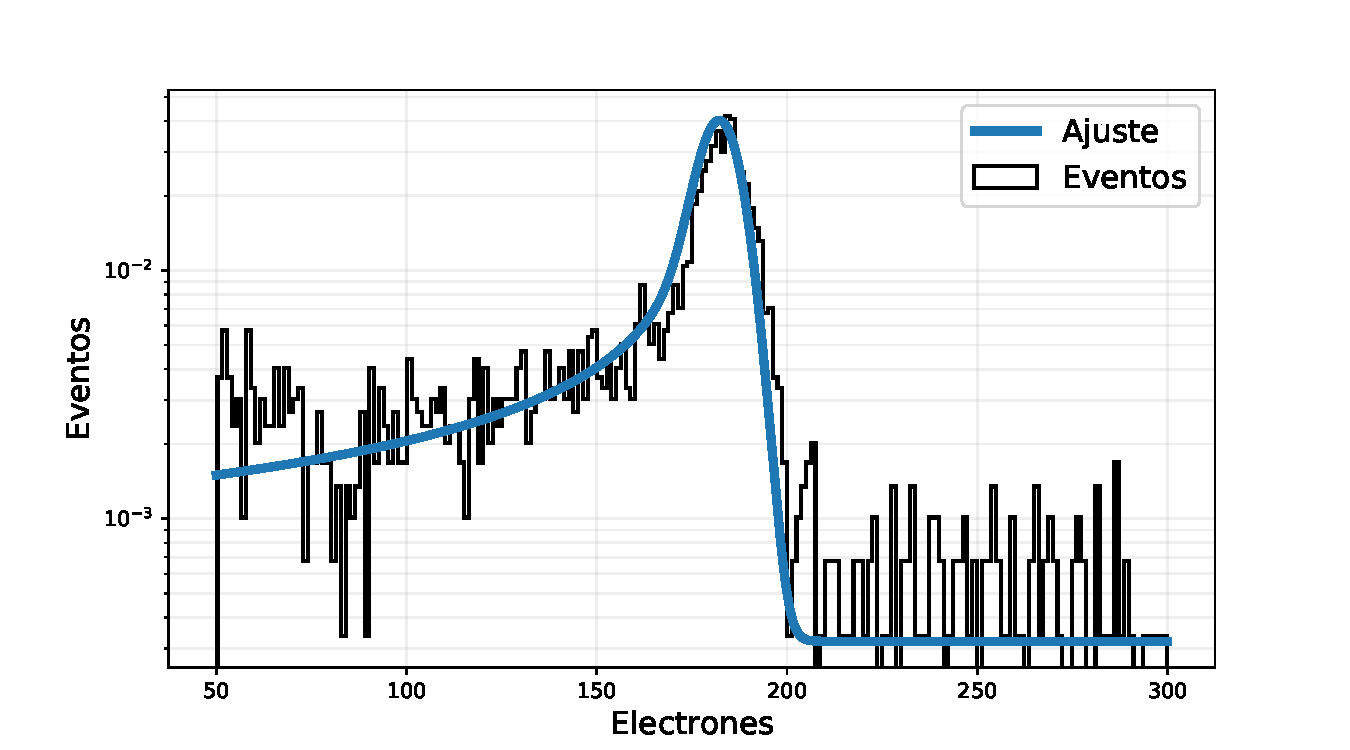
\includegraphics[scale=0.5]{Figs/HistFit_F_EPIX05_OHDU1.pdf}
    \caption{\footnotesize{\textbf{completar}}}
    \label{fig:F_OHDU0_EPIX05}
\end{figure}
De este ajuste se desprenden los valores de los parámetros de interés que son $\beta = 0.0078 \pm 0.0065$, el factor de Fano $F = 0.1480 \pm 0.0123$ y la energía de creación electrón hueco $\varepsilon_{\eh} = 3.6948 \pm 0.0054$.

El segundo paso del análisis se muestra en el gráfico de la Figura \ref{fig:F_OHDU0_EPIX15conCorr}, donde se encuentra el ajuste de los datos para el caso en el que se utilizó el umbral \verb|EPIX=1.5| sin aplicar correcciones. El conteo de eventos en este caso fue de $1812$.
\begin{figure}[h]
    \centering
        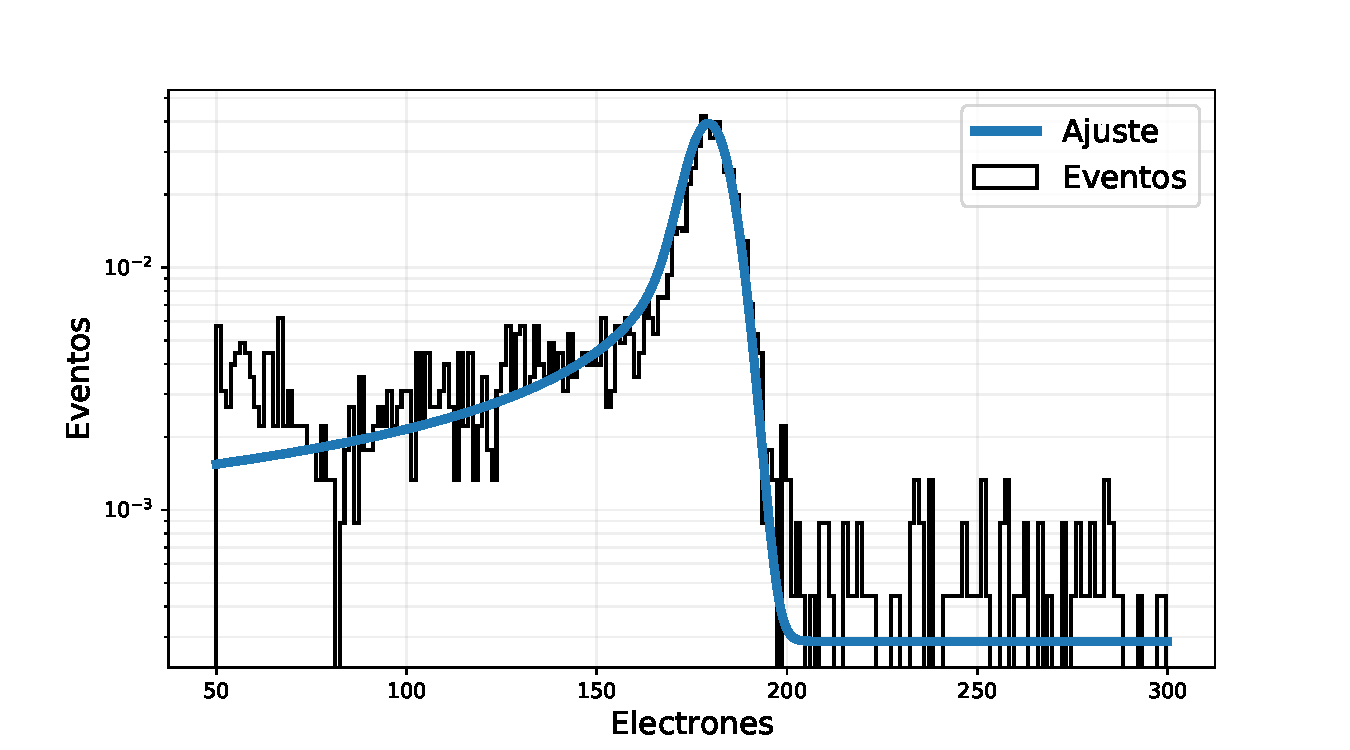
\includegraphics[scale=0.5]{Figs/HistFit_F_EPIX15_OHDU1.pdf}
    \caption{\footnotesize{\textbf{completar}}}
    \label{fig:F_OHDU0_EPIX15sinCorr}
\end{figure}
En este caso se tiene un apreciable aumento de $\beta$, obteniéndose $\beta = 0.0104 \pm 0.0055$, lo cual también es apreciable en el gráfico porque se observa mayor incidencia de eventos en la cola izquierda del pico. El factor de Fano resultó $F = 0.1553 \pm 0.0159$ y la energía de creación electrón hueco $\eh = 3.7516 \pm 0.0079$. Las incertezas de todos estos parámetros se redujeron sensiblemente respecto al caso anterior con menor estadística. Para el caso de los valores de los parámetros, el factor de Fano disminuyó, mientras que la energía de creación electrón hueco aumentó.

En el tercer paso, utilizando \verb|EPIX = 1.5| y las correcciones obtenidas de los análisis previos, se obtuvo el ajuste que se ven el gráfico de la Figura \ref{fig:F_OHDU0_EPIX15conCorr}. Este es muy similar al anterior, dado que el cambio más significativo es el aumento en la estadística mientras que las correcciones no introducen cambios visibles en los histogramas. El conteo de eventos resultó sutilmente menor al caso anterior, $1806$ lo cual resulta \textbf{inesperadoooooo}
\begin{figure}[h]
    \centering
        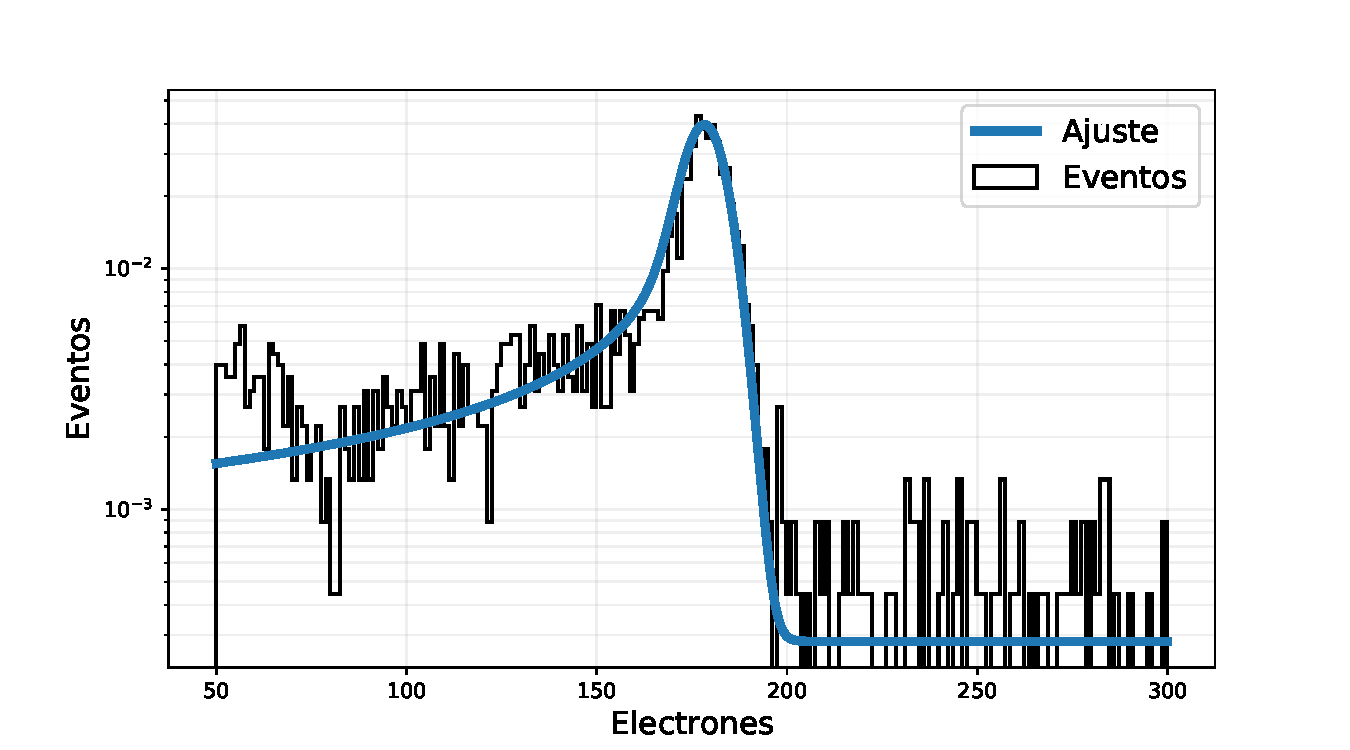
\includegraphics[scale=0.5]{Figs/HistFit_F_EPIX15_OHDU1_Corr.pdf}
    \caption{\footnotesize{\textbf{completar}}}
    \label{fig:F_OHDU0_EPIX15conCorr}
\end{figure}
En cuanto a los parámetros, el valor del $\beta$ aumentó sensiblemente respecto al caso sin correciones, teniéndose $\beta = 0.0111 \pm 0.0062$. El factor de Fano disminuyó aún más, siendo $F = 0.1535 \pm 0.0157$ donde también disminuyó su incerteza. La energía de creación electrón hueco por su parte aumentó siendo $\varepsilon_{\eh} = 3.7744 \pm 0.0076$ y su incerteza también aumento ligeramente respecto al caso sin correciones.

Los resultados de estos mismos análisis para el resto de los cuadrantes se condensas en las Tablas \ref{tab:F_FanoEehOHDU1y2} y \ref{tab:F_FanoEehOHDU3y4}

\begin{table}[H]
\centering
\begin{tabular}{@{}ccccc@{}}
\toprule
                & Eventos                 & $\beta$ & $F$                 & $\varepsilon_{\eh}$ \\ \hline \hline
EPIX 0.5 & $677$ & $0.0078 \pm 0.0065$ & $0.1302 \pm 0.0216$ & $3.5195 \pm 0.0193$  \\
EPIX 1.5 & $1977$ & $0.0104 \pm 0.0055$ & $0.1225 \pm 0.0114$ & $3.5867 \pm 0.0111$\\
EPIX 1.5 Corr & $1972$ & $0.0111 \pm 0.0062$ & $0.1192 \pm 0.0110$ & $3.6069 \pm 0.0113$ \\ \bottomrule
\end{tabular}
\caption{tabla}
\label{tab:F_FanoEehBetaEventos}
\end{table}


\begin{table}[H]
\centering
\begin{tabular}{@{}ccccc@{}}
\toprule
                & \multicolumn{2}{c}{OHDU1}                 & \multicolumn{2}{c}{OHDU2}                 \\ \hline\hline
                & $F$                 & $\varepsilon_{\eh}$ & $F$                 & $\varepsilon_{\eh}$ \\
EPIX 0.5 & $0.1302 \pm 0.0216$ & $3.5195 \pm 0.0193$ & $0.xxxx \pm 0.xxxx$ & $3.xxxx \pm 0.xxxx$ \\
EPIX 1.5 & $0.1225 \pm 0.0114$ & $3.5867 \pm 0.0111$ & $0.xxxx \pm 0.xxxx$ & $3.xxxx \pm 0.xxxx$ \\
EPIX 1.5 Corr & $0.1192 \pm 0.0110$ & $3.6069 \pm 0.0113$ & $0.xxxx \pm 0.xxxx$ & $3.xxxx \pm 0.xxxx$ \\ \bottomrule
\end{tabular}
\caption{tabla}
\label{tab:F_FanoEehOHDU1y2}
\end{table}


\begin{table}[H]
\centering
\begin{tabular}{@{}ccccc@{}}
\toprule
                & \multicolumn{2}{c}{OHDU3}                 & \multicolumn{2}{c}{OHDU4}                 \\ \hline\hline
                & $F$                 & $\varepsilon_{\eh}$ & $F$                 & $\varepsilon_{\eh}$ \\
EPIX 0.5 & $0.xxxx \pm 0.xxxx $ & $3.xxxx \pm 0.xxxx $ & $0.xxxx \pm 0.xxxx $ & $3.xxxx \pm 0.xxxx $ \\ 
EPIX 1.5 & $0.xxxx \pm 0.xxxx $ & $3.xxxx \pm 0.xxxx $ & $0.xxxx \pm 0.xxxx $ & $3.xxxx \pm 0.xxxx $ \\ 
EPIX 1.5 Corr& $0.xxxx \pm 0.xxxx $ & $3.xxxx \pm 0.xxxx$ & $0.xxxx \pm 0.xxxx $ & $3.xxxx \pm 0.xxxx $ \\ \bottomrule
\end{tabular}
\caption{tabla}
\label{tab:F_FanoEehOHDU3y4}
\end{table}


\subsection{Aluminio}
\noindent Para el caso del pico del aluminio se presentan los resultados de igual manera que para los de flúor. Primero sin aplicar el nuevo umbral, luego aplicando \verb|EPIX = 1.5| sin correcciones y por último \verb|EPIX = 1.5| con las correcciones, siempre tomando el primer cuadrante del sensor y finalmente resumiendo los resultados para los demás cuadrantes en una tablas.

Para el primero de estos pasos puede verse el histograma de carga y su respectivo ajuste en la Figura \ref{fig:Al_OHDU1_EPIX05}, del cual se obtiene un valor para el factor de Fano de $F = 0.1322 \pm 0.0022$ y la energía de creación electrón hueco $\varepsilon_{\eh} = 3.7141 \pm 0.0019$
\begin{figure}[H]
    \centering
        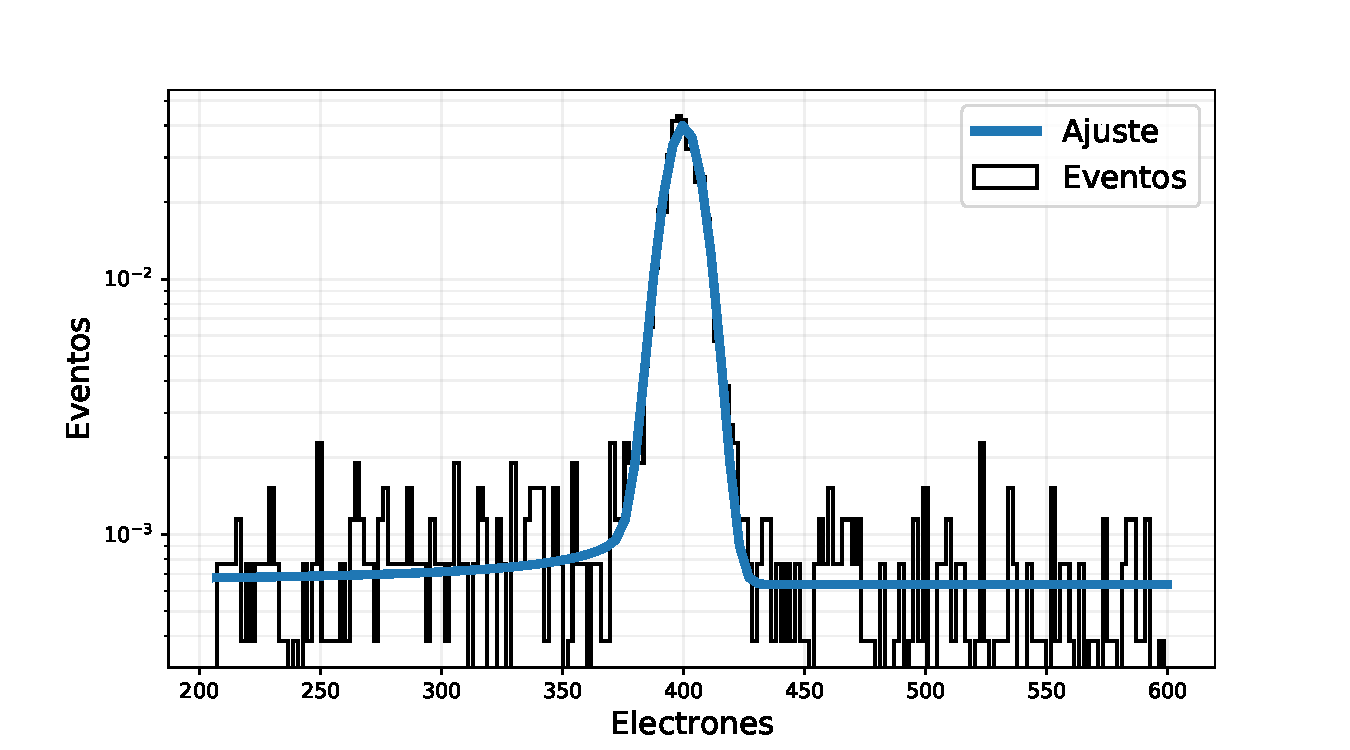
\includegraphics[scale=0.5]{Figs/HistFit_EPIX05_OHDU1_SinCorr.pdf}
    \caption{\footnotesize{asd.}}
    \label{fig:Al_OHDU1_EPIX05}
\end{figure}

El histograma y ajuste del pico del aluminio para el segundo paso del análisis se puede ver en la Figura \ref{fig:Al_OHDU1_EPIX15_SinCorr}. El valor del factor de Fano obtenido es $F = 0.1455 \pm 0.0098$ y para la energía de creación electrón-hueco $\varepsilon_{\eh} = 3.7379 \pm 0.0024$. Lo primero que se observa es que la incerteza del factor de Fano aumenta levemente lo cual es un resultado inesperado debido al aumento en la estadística luego de aplicar el umbral. Mismo caso para la energía de creación electrón hueco, donde la incerteza obtenida aumenta sutilmente. Los magnitudes también difieren entre sí más allá de sus errores, un $\sim 10\,\%$ para el factor de Fano y menos del $1\,\%$ para la energía de creación electrón hueco.
\begin{figure}[H]
    \centering
        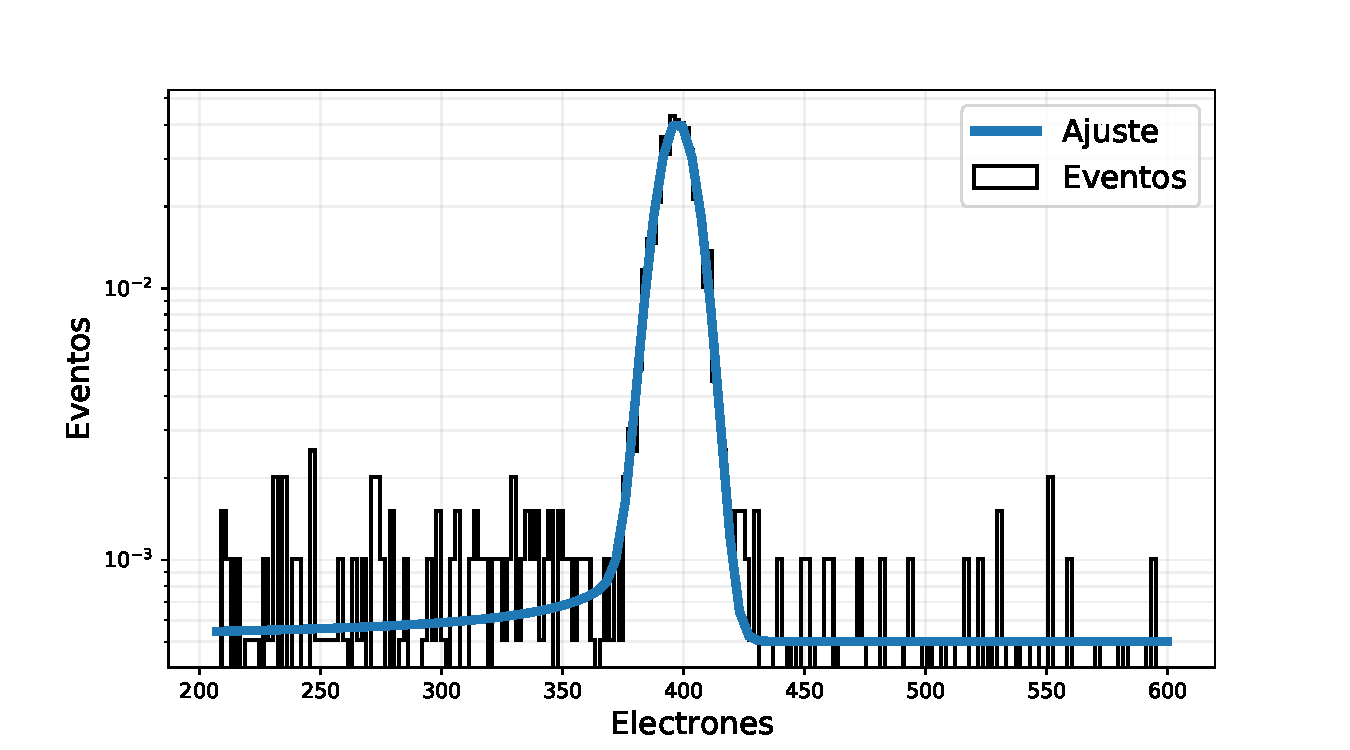
\includegraphics[scale=0.5]{Figs/HistFit_100c_EPIX15_OHDU1_SinCorr.pdf}
    \caption{\footnotesize{asd.}}
    \label{fig:Al_OHDU1_EPIX15_SinCorr}
\end{figure}

Por último, cuando se aplican tanto el umbral \verb|EPIX = 1.5| como las correcciones en el programa y se generan los ajustes a los histogramas de carga, se obtiene que el factor de Fano es $F = 0.1450 \pm 0.0037$ y la energía de creación electrón hueco $\varepsilon_{\eh} = 3.7501 \pm 0.0006$. En efecto, se obtienen ligeras variaciones en los valores para el factor de Fano y la energía de creación electrón hueco. En cuanto a las incertezas, estas disminuyen bastante respecto a las anteriormente calculadas y, en particular, la incerteza de la energía de creación electrón hueco es demasiado pequeña.
\begin{figure}[H]
    \centering
        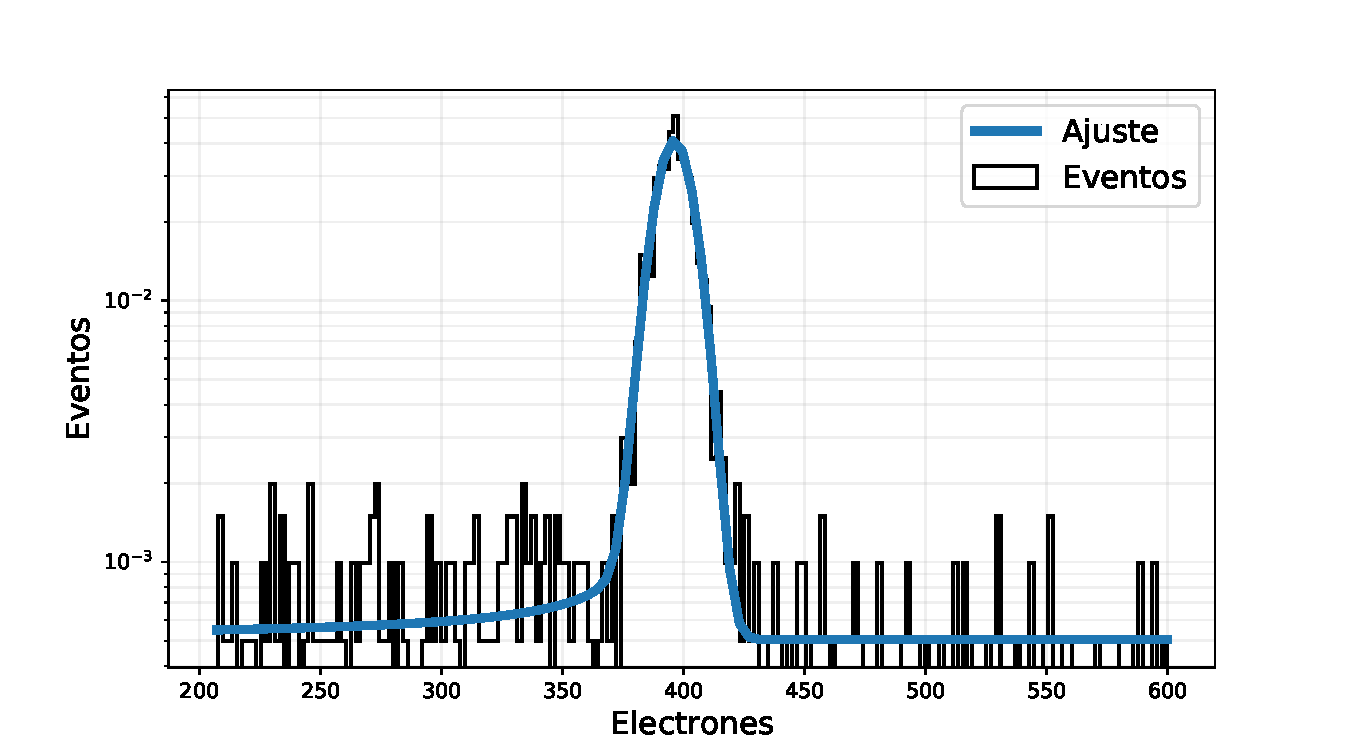
\includegraphics[scale=0.5]{Figs/HistFit_100c_EPIX15_OHDU1_Corr.pdf}
    \caption{\footnotesize{asd.}}
    \label{fig:Al_OHDU1_EPIX15_Corr}
\end{figure}
Al igual que para el caso del flúor, en las Tablas \ref{tab:FanoEehOHDU1y2} y \ref{tab:FanoEehOHDU3y4} se condensan los resultados obtenidos para los demás cuadrantes.

Es importante destacar que para el caso del aluminio, no se observan diferencias apreciables en los ajustes para los diferentes análisis realizados sobre los datos. Por otro lado, también resulta relevante notar la diferencia en el efecto de la colección parcial de carga entre el flúor y el aluminio, donde para el primero las colas a la izquierda del pico son mucho más pronunciadas que para el aluminio. Esto se debe a que el valor de $\beta$ para el flúor resulta aproximadamente $8$ veces mayor que para el aluminio, con lo cual, hay mucha más carga que sufre recombinación producto de la PCC.
\begin{table}[H]
\centering
\begin{tabular}{@{}ccccc@{}}
\toprule
                & \multicolumn{2}{c}{OHDU1}                 & \multicolumn{2}{c}{OHDU2}                 \\ \hline\hline
                & $F$                 & $\varepsilon_{\eh}$ & $F$                 & $\varepsilon_{\eh}$ \\
EPIX 0.5 & $0.1322 \pm 0.0022$ & $3.7141 \pm 0.0019$ & $0.1401 \pm 0.0117$ & $3.7149 \pm 0.0037$ \\ \hline
EPIX 1.5 50c & $0.1418 \pm 0.0148$ & $3.7399 \pm 0.0044$ & $0.1339 \pm 0.0186$ & $3.7532 \pm 0.0059$ \\
EPIX 1.5 100c & $0.1455 \pm 0.0098$ & $3.7379 \pm 0.0024$ & $0.1530 \pm 0.0000$ & $3.7386 \pm 0.000$ \\ \hline
EPIX 1.5 50c Corr & $0.1406 \pm 0.0000$ & $3.7490 \pm 0.0000$ & $0.1353 \pm 0.0187$ & $3.7421 \pm 0.0059$ \\
EPIX 1.5 100c Corr & $0.1450 \pm 0.0037$ & $3.7501 \pm 0.0006$ & $0.1513 \pm 0.2640$ & $3.7270 \pm 0.0799$ \\ \bottomrule \hline
\end{tabular}
\caption{tabla}
\label{tab:FanoEehOHDU1y2}
\end{table}
\begin{table}[H]
\centering
\begin{tabular}{@{}ccccc@{}}
\toprule
                & \multicolumn{2}{c}{OHDU3}                 & \multicolumn{2}{c}{OHDU4}                 \\ \hline\hline
                & $F$                 & $\varepsilon_{\eh}$ & $F$                 & $\varepsilon_{\eh}$ \\
EPIX 0.5 & $0.1498 \pm 0.00101$ & $3.7209 \pm 0.0029$ & $0.1812 \pm 0.0166$ & $3.7305 \pm 0.0041$ \\ \hline
EPIX 1.5 50c & $0.1548 \pm 0.0001$ & $3.7449 \pm 0.0000$ & $0.1601 \pm 0.3691$ & $3.7633 \pm 0.1139$ \\
EPIX 1.5 100c & $0.1699 \pm 0.0150$ & $3.7419 \pm 0.0039$ & $0.1931 \pm 0.0208$ & $3.7541 \pm 0.0000$ \\ \hline
EPIX 1.5 50c  Corr& $0.1538 \pm 0.0000$ & $3.7510 \pm 0.0000$ & $0.1487 \pm 0.0000$ & $3.7698 \pm 0.0000$ \\
EPIX 1.5 100c Corr& $0.1701 \pm 0.0141$ & $3.7485 \pm 0.0039$ & $0.1933 \pm 0.0194$ & $3.7634 \pm 0.0047$ \\ \bottomrule \hline
\end{tabular}
\caption{tabla}
\label{tab:FanoEehOHDU3y4}
\end{table}

%%%%%%%%%%%%%%%%%%%%%%%%%%%%%%%%%%%%%%%%%%%%%%%%%%%%%%%%%%%%%%%%%%
%%%%%%%%%%%%%%%%%%%%%%%%%%%%%%%%%%%%%%%%%%%%%%%%%%%%%%%%%%%%%%%%%%
\section{Valores de \texorpdfstring{$\beta$}{beta}}
\noindent Los valores del parámetro $\beta$ junto con su error se determinaron utilizando el método de la máxima verosimilitud como se detalla en la sección \ref{sec:MaximaVerosimilitud}. De realizar este procedimiento se obtuvo el gráfico de la verosimilitud que se ve en la Figura \ref{fig:LL_beta} y que se ajustó con una función cuadrática para \textbf{para qué?}. Se puede observar la intersección entre la recta que se encuentra a una distancia $a=1/2$ por debajo del máximo y la curva obtenida del barrido en $\beta$ para la verosimilitud. De estos se obtuvo el intervalo $[0.00396, 0.01144]$ para un $68.3\,\%$ de probabilidad de contener a $beta$, para el \textbf{cual?} cuadrante del sensor y el caso de los rayos $X$ del aluminio.
\begin{figure}[H]
    \centering
        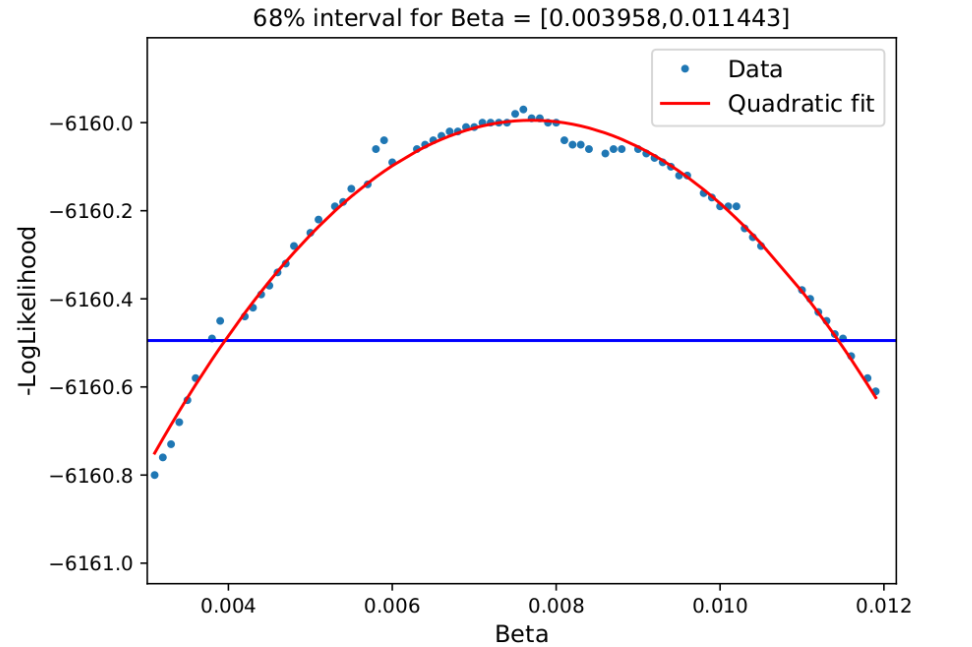
\includegraphics[scale=0.4]{pngs/LL_beta.png}
    \caption{\footnotesize{asd.}}
    \label{fig:LL_beta}
\end{figure}
\textcolor{red}{\textbf{\textit{Para seguir con la lógica de mostrar los resultados de cada uno de los 3 pasos, necesitaría este mismo gráfico para cada uno de esos pasos, además de necesitar el del flúor, porque entiendo que este es el del aluminio.}}}
También se logra observar lo que se esperaba respecto a la intensidad de del parámetro $\beta$: Para los picos de los rayos $X$ del flúor, las colas en los picos de los histogramas son apreciablemente más pronunciadas que para los picos de los rayos $X$ del aluminio. Esto se debe a que $\beta_{F} = 0.008$ mientras que $\beta_{Al} = 0.001$, siendo el efecto de la PCC 8 veces más pronunciado para el caso del flúor.

\begin{figure}[H]
    \centering
        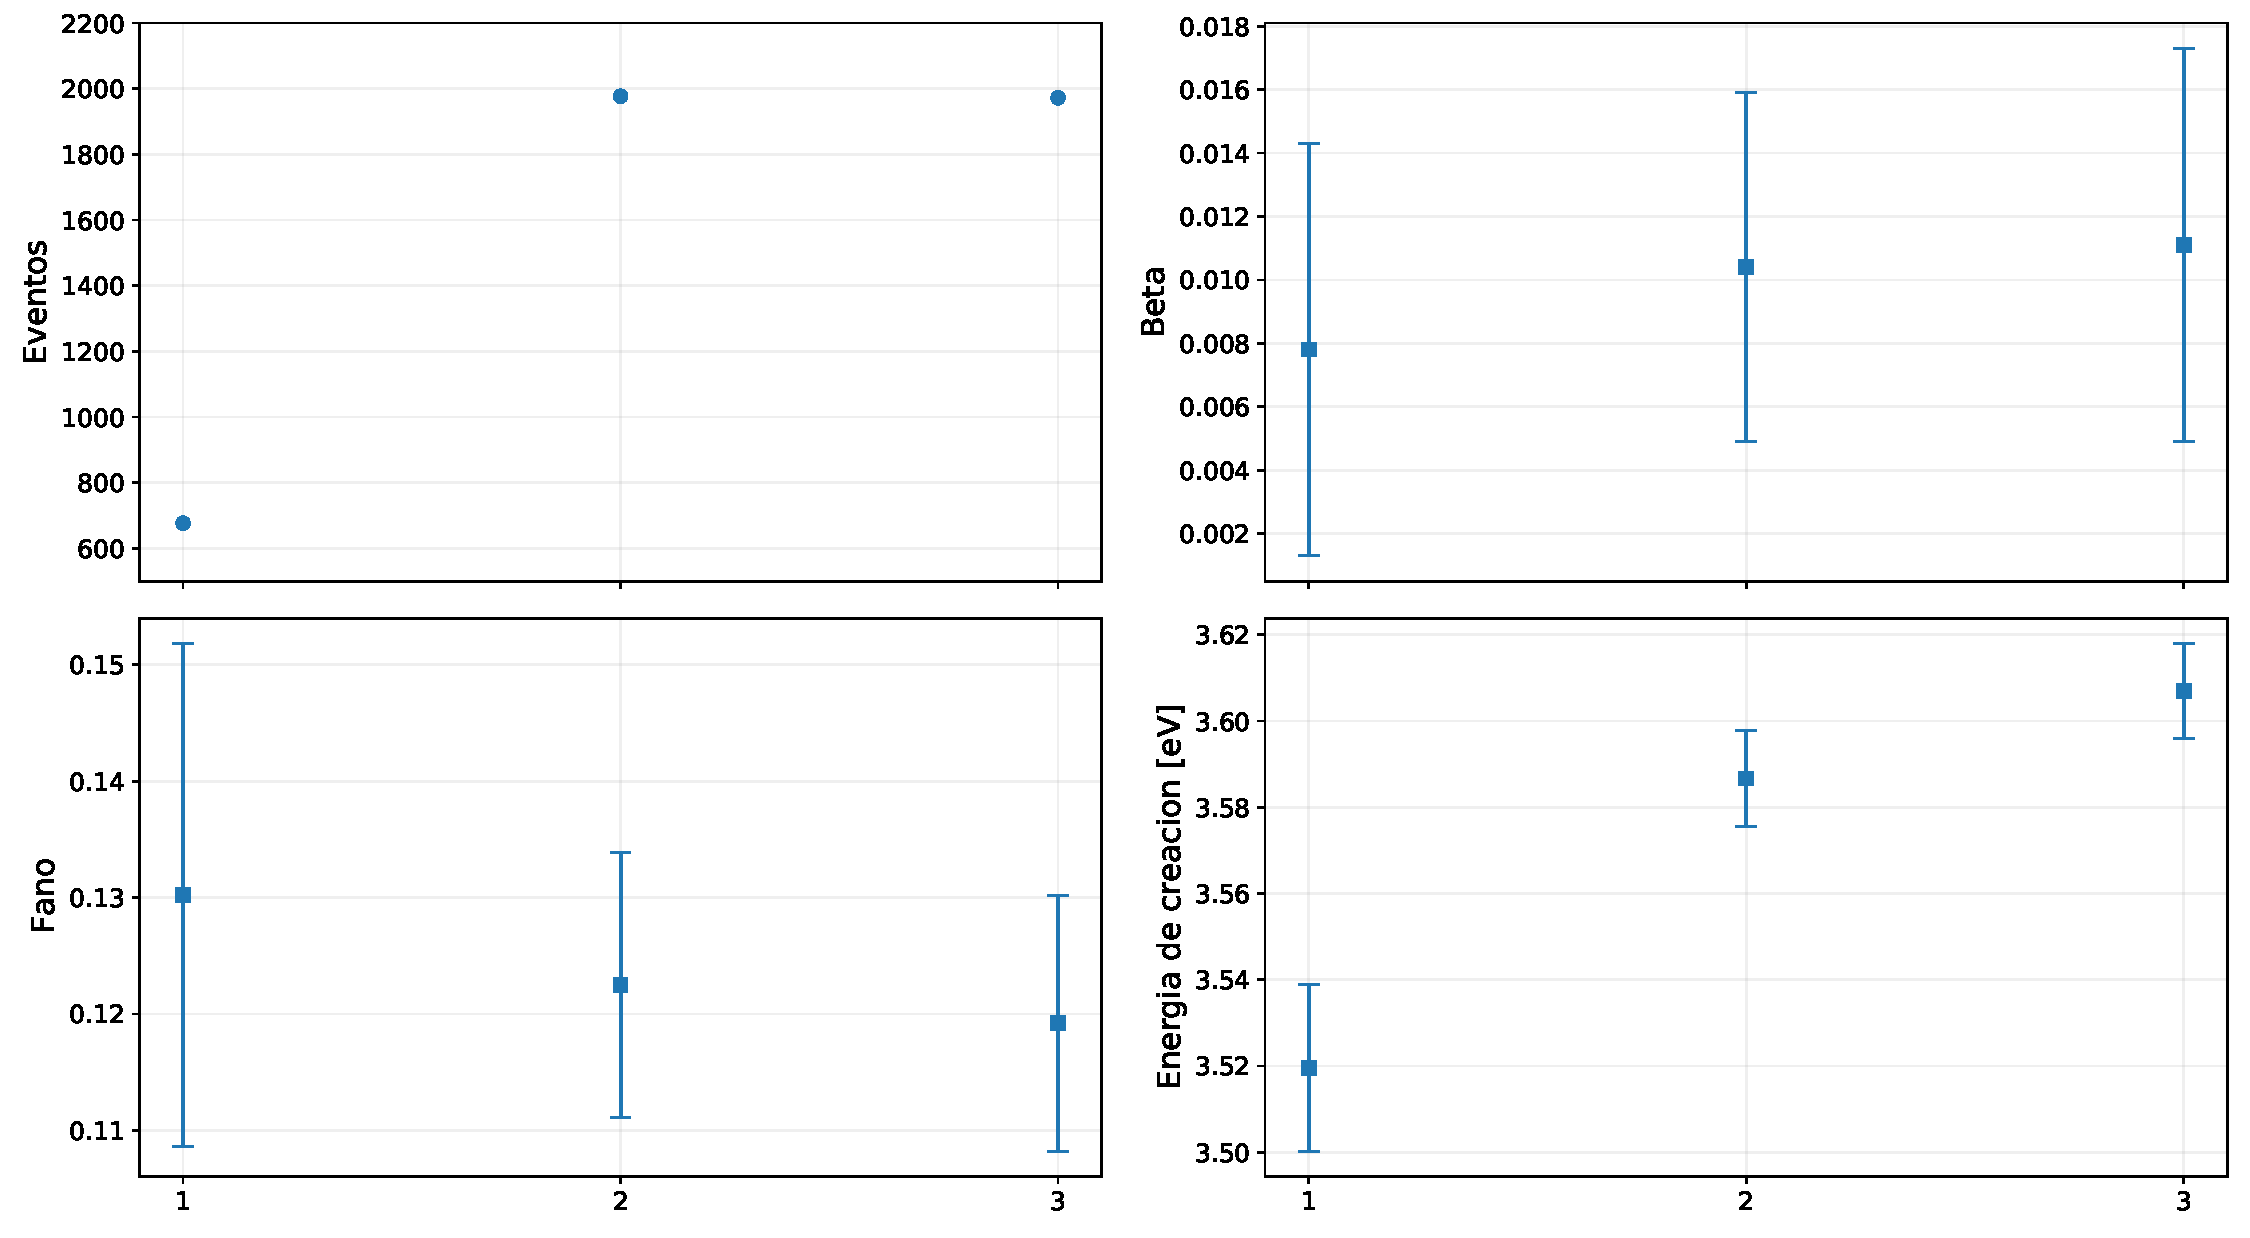
\includegraphics[scale=0.45]{Figs/F_OHDU1_EventosBetaFanoEH.pdf}
    \caption{\footnotesize{Resultados para cada uno de los pasos de análisis para el flúor y el primer cuadrante. Se presentan la cantidad de eventos registrados, el valor del parámetro $\beta$, el factor de Fano y la energía de creación electrón hueco. AGREGAR QUE SIGNIFICA 1, 2, Y 3}}
    \label{fig:F_OHDU1_EventosBetaFanoEH}
\end{figure}
\textcolor{red}{EL BETA NO IMPORTA, IMPORTA EL TAMAÑO DE LA PCC $\beta\tau_{CCE}$}
ENERGIA DE CREACIÓN HUECO, FANO Y TAU (tamaño de la pcc) en un gráfico de $1x3$ (uno arriba del otro, no apaisado)
\begin{figure}[H]
    \centering
        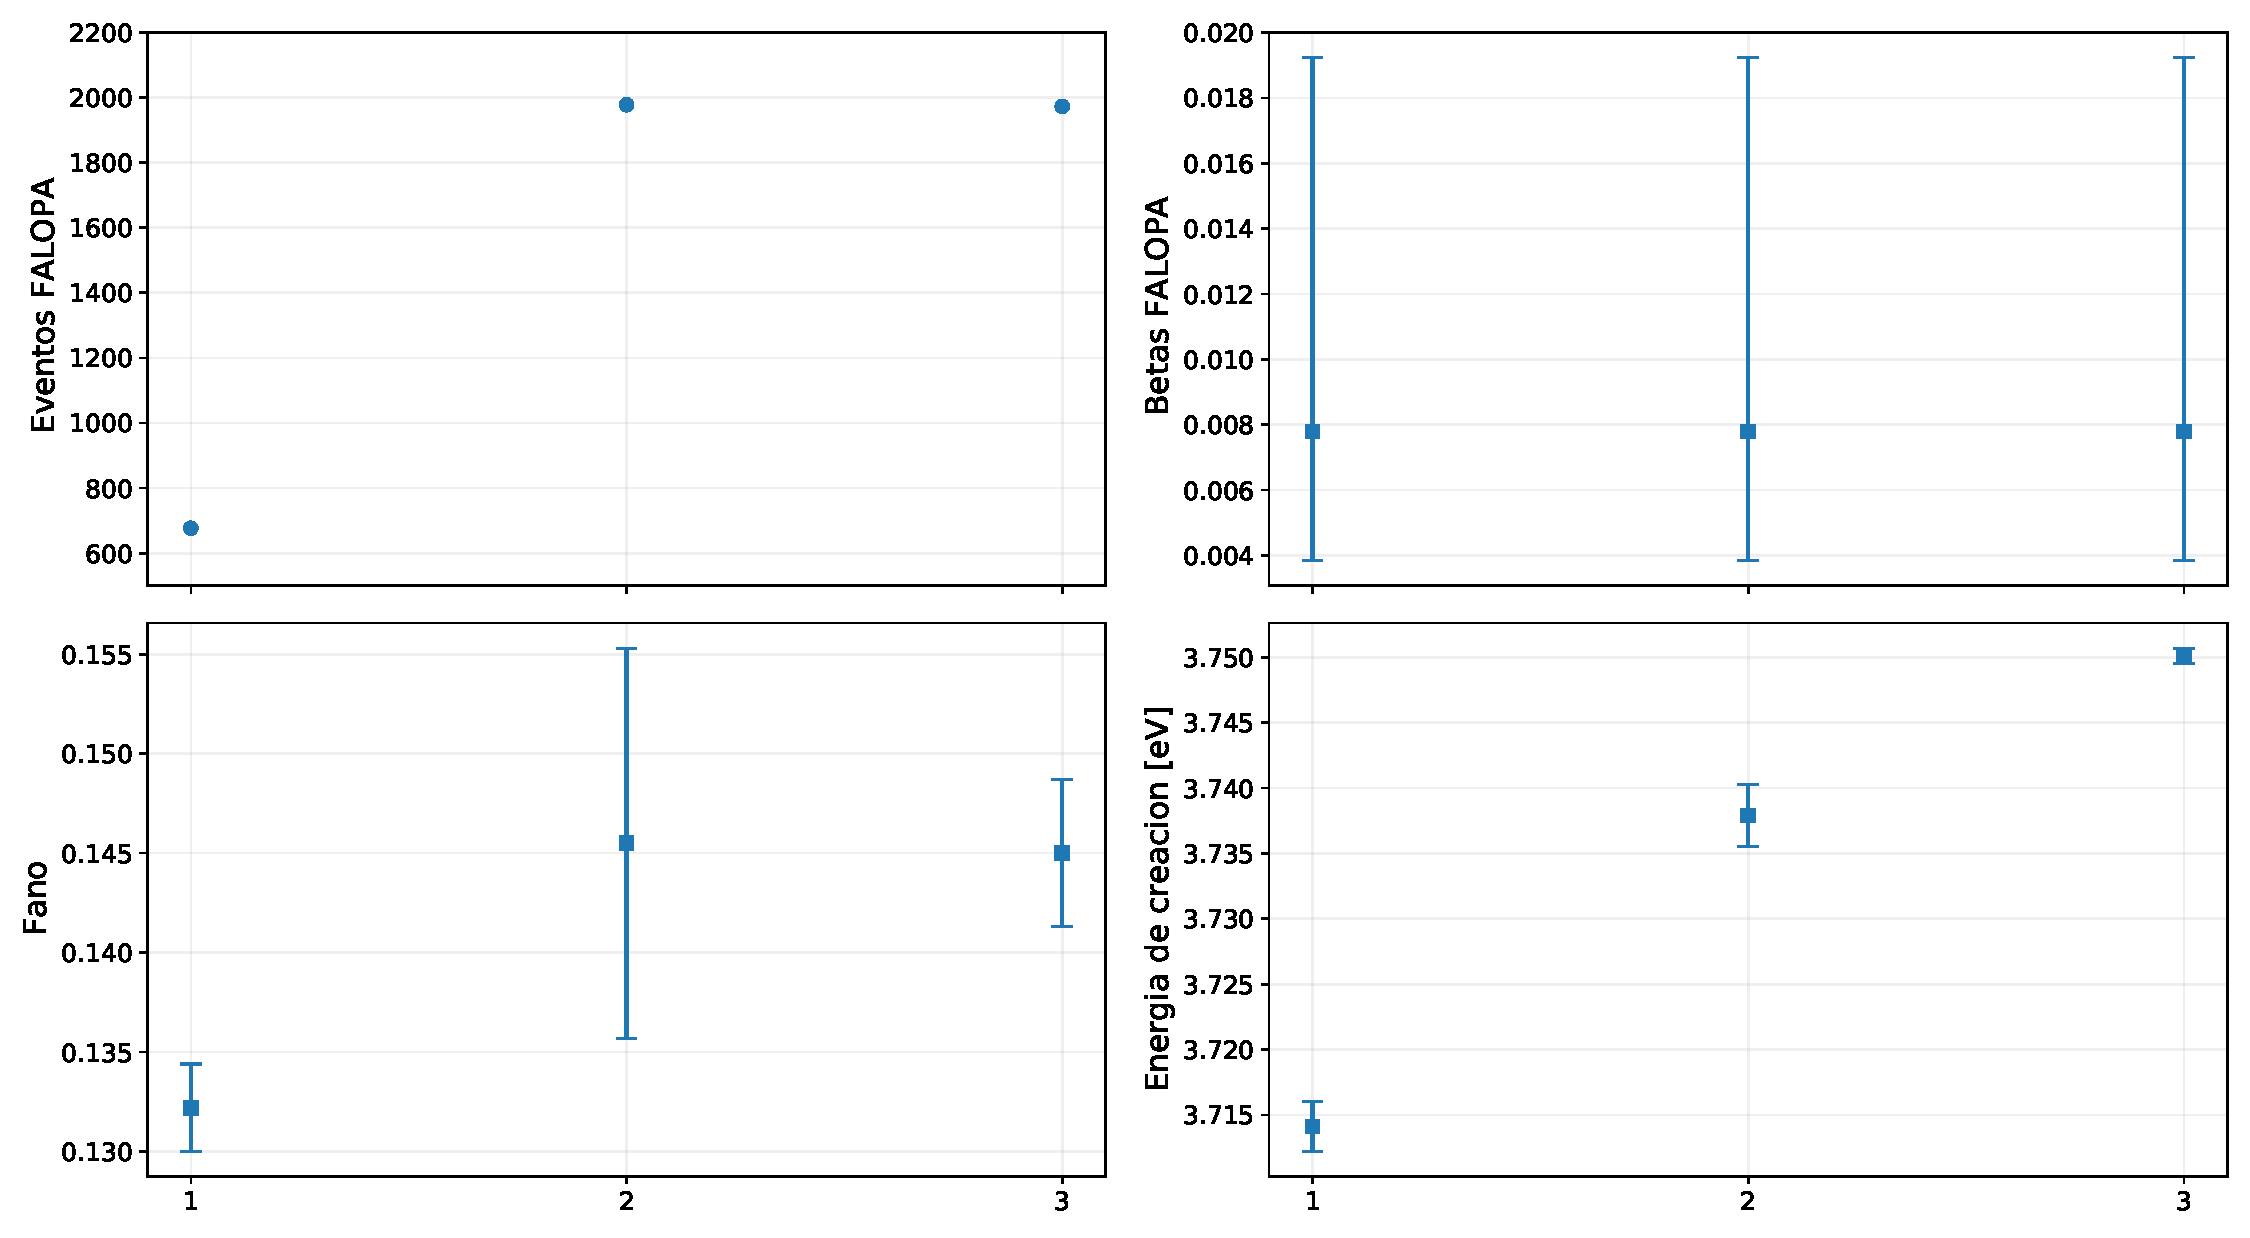
\includegraphics[scale=0.45]{Figs/Al_OHDU1_EventosBetaFanoEH.pdf}
    \caption{\footnotesize{Resultados para cada uno de los pasos de análisis para el aluminio y el primer cuadrante. Se presentan la cantidad de eventos registrados, el valor del parámetro $\beta$, el factor de Fano y la energía de creación electrón hueco.\textcolor{red}{Acá puse la misma cantidad de eventos que los del flúor, porque los del aluminio no los tengo, no sé qué parte del codigo los printea en pantalla. También puse 3 veces el mismo valor de beta con sus intervalos porque no los tengo para el caso EPIX 0.5, EPIX 1.5 sin correcciones. En teoría este es para EPIX 1.5 con correcciones.}}}
    \label{fig:Al_OHDU1_EventosBetaFanoEH}
\end{figure}